\documentclass[tikz,border=5pt]{standalone}
\usepackage{tikz}
\usetikzlibrary{shapes.geometric,arrows.meta,positioning,fit,backgrounds,shadows,decorations.pathreplacing,calc}

\begin{document}
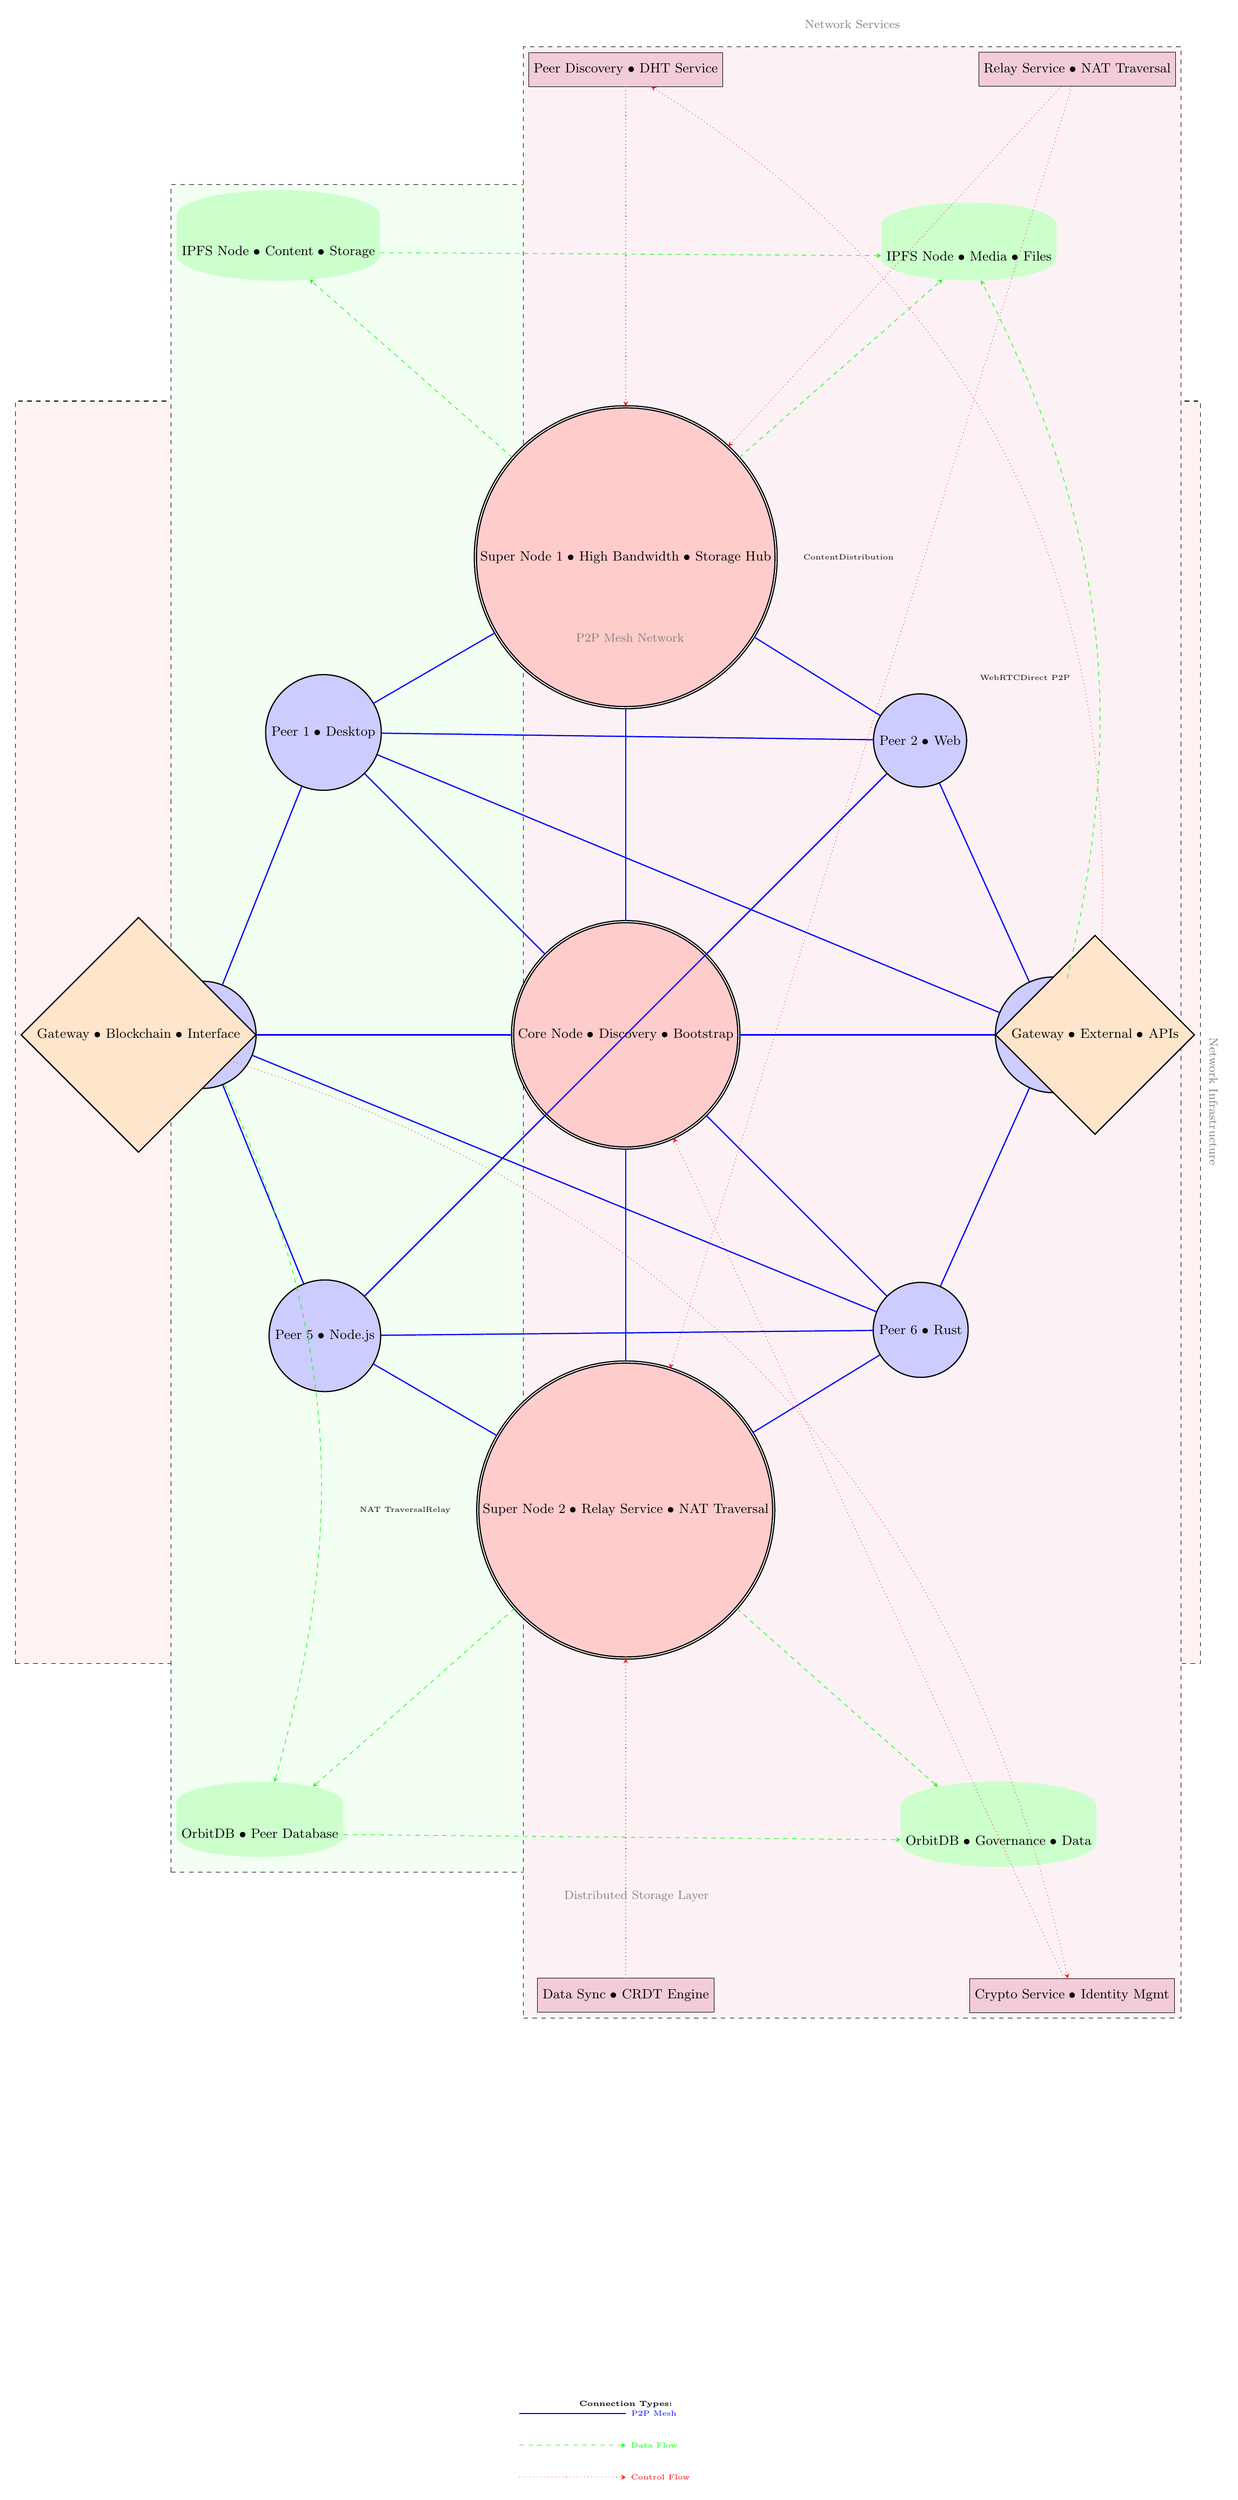
\begin{tikzpicture}[scale=2.5,
    node distance=6cm,
    every node/.style={font=\small},
    % Node types
    peer/.style={circle,draw,minimum size=1.2cm,fill=blue!20,thick},
    supernode/.style={circle,draw,minimum size=1.6cm,fill=red!20,thick,double},
    gateway/.style={diamond,draw,minimum size=1.2cm,fill=orange!20,thick},
    storage/.style={cylinder,shape border rotate=90,aspect=0.25,minimum height=1cm,minimum width=1.4cm,fill=green!20},
    service/.style={rectangle,draw,minimum width=1.6cm,minimum height=0.8cm,fill=purple!20},
    arrow/.style={->,>=stealth,thick},
    p2p_connection/.style={-,thick,blue},
    data_flow/.style={->,>=stealth,dashed,green},
    control_flow/.style={->,>=stealth,dotted,red}
]

% Central Network Core
\node[supernode] (core_node) {Core Node • Discovery • Bootstrap};

% Peer Nodes in Mesh Formation
\node[peer,above left=of core_node] (peer1) {Peer 1 • Desktop};
\node[peer,above right=of core_node] (peer2) {Peer 2 • Web};
\node[peer,left=of core_node] (peer3) {Peer 3 • Mobile};
\node[peer,right=of core_node] (peer4) {Peer 4 • Desktop};
\node[peer,below left=of core_node] (peer5) {Peer 5 • Node.js};
\node[peer,below right=of core_node] (peer6) {Peer 6 • Rust};

% Super Nodes for Network Optimization
\node[supernode,above=5cm of core_node] (supernode1) {Super Node 1 • High Bandwidth • Storage Hub};
\node[supernode,below=5cm of core_node] (supernode2) {Super Node 2 • Relay Service • NAT Traversal};

% Gateway Nodes for Cross-Network Communication
\node[gateway,left=6cm of core_node] (gateway1) {Gateway • Blockchain • Interface};
\node[gateway,right=6cm of core_node] (gateway2) {Gateway • External • APIs};

% Distributed Storage Nodes
\node[storage,above left=4cm and 5cm of supernode1] (ipfs1) {IPFS Node • Content • Storage};
\node[storage,above right=4cm and 5cm of supernode1] (ipfs2) {IPFS Node • Media • Files};
\node[storage,below left=4cm and 5cm of supernode2] (orbitdb1) {OrbitDB • Peer Database};
\node[storage,below right=4cm and 5cm of supernode2] (orbitdb2) {OrbitDB • Governance • Data};

% Services Layer
\node[service,above=7.5cm of supernode1] (discovery) {Peer Discovery • DHT Service};
\node[service,right=of discovery] (relay) {Relay Service • NAT Traversal};
\node[service,below=7.5cm of supernode2] (sync) {Data Sync • CRDT Engine};
\node[service,right=of sync] (crypto) {Crypto Service • Identity Mgmt};

% Background Network Zones
\begin{scope}[on background layer]
% Mesh Network Zone
\node[fill=blue!5,draw,dashed,fit=(peer1)(peer2)(peer3)(peer4)(peer5)(peer6)(core_node)] (mesh_zone) {};

% Infrastructure Zone
\node[fill=red!5,draw,dashed,fit=(supernode1)(supernode2)(gateway1)(gateway2)] (infra_zone) {};

% Storage Zone
\node[fill=green!5,draw,dashed,fit=(ipfs1)(ipfs2)(orbitdb1)(orbitdb2)] (storage_zone) {};

% Services Zone
\node[fill=purple!5,draw,dashed,fit=(discovery)(relay)(sync)(crypto)] (services_zone) {};
\end{scope}

% Mesh P2P Connections
\draw[p2p_connection] (core_node) -- (peer1);
\draw[p2p_connection] (core_node) -- (peer2);
\draw[p2p_connection] (core_node) -- (peer3);
\draw[p2p_connection] (core_node) -- (peer4);
\draw[p2p_connection] (core_node) -- (peer5);
\draw[p2p_connection] (core_node) -- (peer6);

% Peer-to-Peer Mesh Connections
\draw[p2p_connection] (peer1) -- (peer2);
\draw[p2p_connection] (peer2) -- (peer4);
\draw[p2p_connection] (peer4) -- (peer6);
\draw[p2p_connection] (peer6) -- (peer5);
\draw[p2p_connection] (peer5) -- (peer3);
\draw[p2p_connection] (peer3) -- (peer1);
\draw[p2p_connection] (peer1) -- (peer4);
\draw[p2p_connection] (peer2) -- (peer5);
\draw[p2p_connection] (peer3) -- (peer6);

% Super Node Connections
\draw[p2p_connection] (core_node) -- (supernode1);
\draw[p2p_connection] (core_node) -- (supernode2);
\draw[p2p_connection] (supernode1) -- (peer1);
\draw[p2p_connection] (supernode1) -- (peer2);
\draw[p2p_connection] (supernode2) -- (peer5);
\draw[p2p_connection] (supernode2) -- (peer6);

% Gateway Connections
\draw[p2p_connection] (core_node) -- (gateway1);
\draw[p2p_connection] (core_node) -- (gateway2);

% Storage Connections
\draw[data_flow] (supernode1) -- (ipfs1);
\draw[data_flow] (supernode1) -- (ipfs2);
\draw[data_flow] (supernode2) -- (orbitdb1);
\draw[data_flow] (supernode2) -- (orbitdb2);
\draw[data_flow] (ipfs1) -- (ipfs2);
\draw[data_flow] (orbitdb1) -- (orbitdb2);

% Service Connections
\draw[control_flow] (discovery) -- (supernode1);
\draw[control_flow] (relay) -- (supernode1);
\draw[control_flow] (relay) -- (supernode2);
\draw[control_flow] (sync) -- (supernode2);
\draw[control_flow] (crypto) -- (core_node);

% Cross-zone Communication
\draw[data_flow] (peer3) to[bend left=20] (orbitdb1);
\draw[data_flow] (peer4) to[bend right=20] (ipfs2);
\draw[control_flow] (gateway1) to[bend left=30] (crypto);
\draw[control_flow] (gateway2) to[bend right=30] (discovery);

% Network Flow Indicators
\node[above right=0.5cm and 0.5cm of peer2,font=\tiny] {WebRTC\\Direct P2P};
\node[right=0.5cm of supernode1,font=\tiny] {Content\\Distribution};
\node[left=0.5cm of supernode2,font=\tiny] {NAT Traversal\\Relay};

% Labels
\node[above=0.5cm of mesh_zone,font=\footnotesize,text=gray] {P2P Mesh Network};
\node[right=0.3cm of infra_zone,font=\footnotesize,text=gray,rotate=-90] {Network Infrastructure};
\node[below=0.3cm of storage_zone,font=\footnotesize,text=gray] {Distributed Storage Layer};
\node[above=0.3cm of services_zone,font=\footnotesize,text=gray] {Network Services};

% Legend
\node[below=9cm of sync,font=\tiny] (legend_title) {\textbf{Connection Types:}};
\draw[p2p_connection,below=0.3cm of legend_title] ($(legend_title.south) + (-1,0)$) -- ($(legend_title.south) + (0,0)$) node[right,font=\tiny] {P2P Mesh};
\draw[data_flow,below=0.1cm of legend_title] ($(legend_title.south) + (-1,-0.3)$) -- ($(legend_title.south) + (0,-0.3)$) node[right,font=\tiny] {Data Flow};
\draw[control_flow,below=0.1cm of legend_title] ($(legend_title.south) + (-1,-0.6)$) -- ($(legend_title.south) + (0,-0.6)$) node[right,font=\tiny] {Control Flow};

\end{tikzpicture}
\end{document}
